%
% LATEXBONES
%
\documentclass[a4paper,11pt,twoside]{article}
\usepackage{graphicx}
\usepackage{amsmath}
\usepackage[english]{babel}
\usepackage[applemac]{inputenc}
\usepackage[colorlinks,bookmarks=false,linkcolor=blue,urlcolor=blue]{hyperref}
\usepackage{subfigure}
\usepackage{here}
\usepackage{wrapfig}
\usepackage{fancyhdr}
\usepackage{dirtytalk}

%drow graph
\usepackage{fancybox}
\usepackage{tikz}
\usepackage{capt-of}

% print code
\usepackage{listings}
\usepackage{algorithm2e}
\usepackage{verbatim}

% push at the bottom
\newenvironment{bottompar}{\par\vspace*{\fill}}{\clearpage}

% landscape
\usepackage{pdflscape}

\paperheight=297mm
\paperwidth=210mm

\setlength{\textheight}{235mm}
\setlength{\topmargin}{-1.2cm} 

\setlength{\parindent}{0pt}

\setlength{\textwidth}{15cm}
\setlength{\oddsidemargin}{0.56cm}
\setlength{\evensidemargin}{0.56cm}

% quotes
\usepackage{framed}
\newcommand*{\signed}[1]{%
  \unskip\hspace*{1em plus 1fill}%
  \nolinebreak[3]\hspace*{\fill}\mbox{#1}
}

\pagestyle{plain}

% --- equations ---
\def \be {\begin{equation}}
\def \ee {\end{equation}}
%\def \dd  {{\rm d}}m

% --- links ---
\newcommand{\mail}[1]{{\href{mailto:#1}{#1}}}
\newcommand{\ftplink}[1]{{\href{ftp://#1}{#1}}}






% ======= Document ======

%----------------------------------------------------------------------------------------
% HEADING SECTIONS
%----------------------------------------------------------------------------------------

% --- header ---
\fancyhead[L]{Applied Data Analysis}
\fancyhead[R]{Summary}

\begin{document}
\begin{titlepage} %Titre
\begin{center}
\newcommand{\HRule}{\rule{\linewidth}{0.5mm}} % Defines a new command for the horizontal lines, change thickness here
\center % Center everything on the page
 
 
 %----------------------------------------------------------------------------------------
% TITLE SECTION
%----------------------------------------------------------------------------------------




\begin{figure} [h] %----------- SubGraph ---------------------
\centerline{
\subfigure{
\includegraphics[height = 2 cm]{./pic/EPFL.png}  }
\subfigure{
\includegraphics[height = 2 cm]{./pic/ADA-logo.png}} 
} 
\end{figure}


\vspace{0.5cm}
%\textsc{\LARGE EPFL}\\[1.5cm] % Name of your university/college
\textsc{\Large School Of Computer And Communication Sciences}\\[0.5cm] % Major heading such as course name
\textsc{\Large }\\% Minor heading such as course title
%\textsc{ \Large Master Semester Project}\\ % Minor heading such as course title


\HRule \\[0.4cm]
{ \huge \bfseries Applied Data Analysis \\Summary}\\[0.4cm] % Title of your document
\HRule \\[1.5cm]

% ---- Lovelace -----
\begin{center}
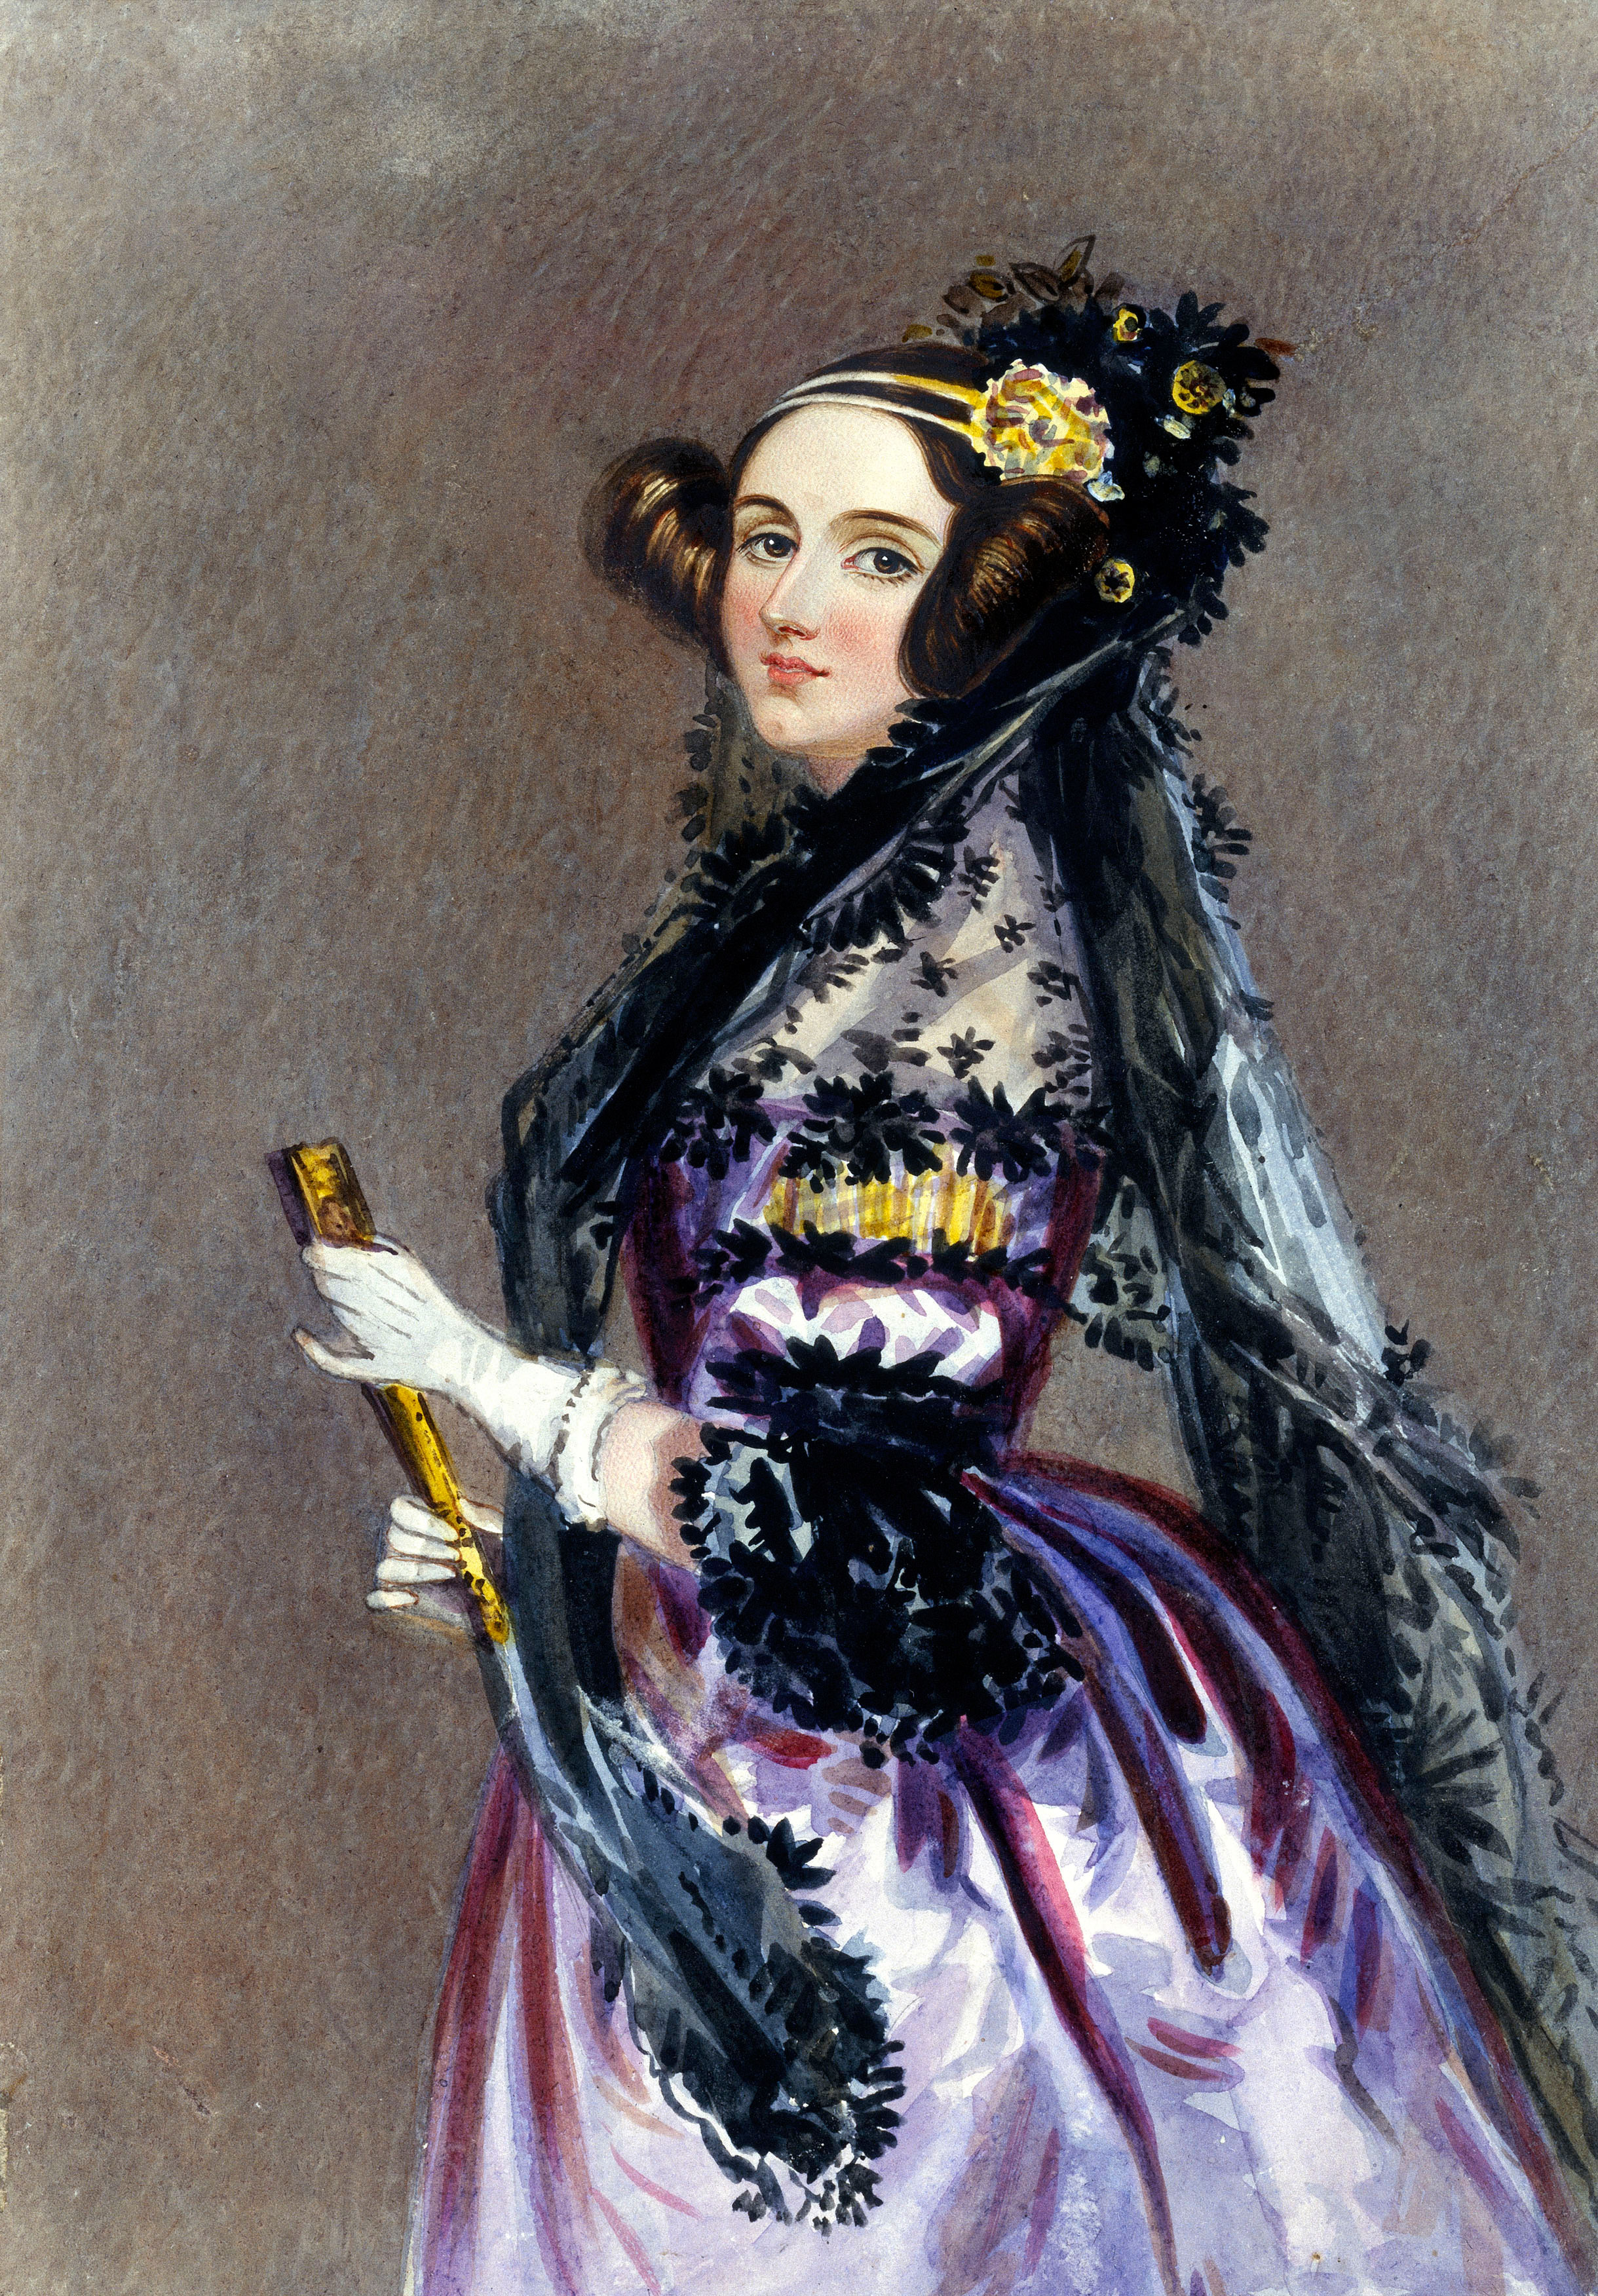
\includegraphics[width = 5 cm]{pic/lovelace} % Include a department/university logo - this will require the graphicx package
\end{center}



\begin{bottompar}
% ---- Professor -----
\begin{flushleft} \large
Prof. \textsc{Catasta} Michele\\
Distributed Information Systems Laboratory (LSIR) \\
\mail{michele.catasta@epfl.ch} \\ 
\end{flushleft}

% ---- date
{\large June 10, 2016}\\[1cm] % Date, change the \today to a set date if you want to be precise

\end{bottompar}
 
%%----------------------------------------------------------------------------------------
%% AUTHOR SECTION
%%----------------------------------------------------------------------------------------

%
%
%
%
%
%\begin{minipage}[t]{0.4\textwidth}
%
%\end{minipage}
%~
%\begin{minipage}[t]{0.55\textwidth}
%%\begin{flushright} \large
%%\emph{Assistant:} \\
%%\textsc{Voirol} Nicolas \\
%%PhD student\\
%%\mail{nicolas.voirol@epfl.ch} \\ [0.4cm]
%%
%%\emph{Supervisor:} \\
%%\textsc{Kuncak} Viktor\\  % Supervisor's Name
%%Professor\\
%%LARA - Laboratory for Automated Reasoning and Analysis\\
%%\mail{viktor.kuncak@epfl.ch}
%%\end{flushright}
%\end{minipage}\\[2cm]

% If you don't want a supervisor, uncomment the two lines below and remove the section above
%\Large \emph{Author:}\\
%John \textsc{Smith}\\[3cm] % Your name

%----------------------------------------------------------------------------------------
% LOGO SECTION
%----------------------------------------------------------------------------------------



%----------------------------------------------------------------------------------------
% DATE SECTION
%----------------------------------------------------------------------------------------

%{\Large \today}\\[1cm] % Date, change the \today to a set date if you want to be precise


%
%\begin{center}
%\abstract{\large Experiment various methods to compare functional trees between them. Given a function, use these algorithms to find the most similar tree contained in a corpus of functions. Try to suggest an autocompletion for a "hole" in a tree, based on this corpus.}
%\end{center} 
 %{\Large IDQ CONFIDENTIAL}
%----------------------------------------------------------------------------------------
\vfill % Fill the rest of the page with whitespace

\end{center}
\end{titlepage}



\pagestyle{fancy}
% ================ Table of content ==============
\newpage
\tableofcontents 

\baselineskip=16pt
%\parindent=15pt
%\parskip=5pt

\newpage




% ================ Introduction ==============
\section{Introduction}

\subsection{General information about the course}

This course covers multiple topics in the data science field such as \textbf{Data Wrangling}, {\bf Data Management}, {\bf Data Mining}, {\bf Machine Learning}, {\bf Visualization}, {\bf Statistics} and {\bf Story telling}. It's about {\bf breadth}, not depth. Indeed, Data science is evolving really quickly, hence learning in depth a specific tool won't pay off. 

\subsection{Data Science}

When we talk about Data Science, we often use the term Big Data as the enormous amount of data that exist in the world. But Big Data is not only about collecting huge amount of data. It is challenging but not enough. The real value comes from the insights. The {\it internet} companies (Google, Facebook, etc.) 
understood this many years ago.
\\ \\
An accurate definition of Data Analysis is given by Wikipedia:
\begin{framed}
{\it {\bf Analysis of data} is a process of {\bf inspecting}, {\bf cleaning}, {\bf transforming}, and {\bf modeling data} with the goal of {\bf discovering useful information}, suggesting conclusions, and supporting decision-making.
Data analysis has multiple facets and approaches, encompassing diverse techniques under a variety of names, {\bf in different business}, science, and social science {\bf domains}.}
\signed{\href{https://en.wikipedia.org/wiki/Data\_analysis}{Wikipedia - Data Analysis}}
\end{framed}

Therefore, a Data Scientist has to master different kind of skills such as {\bf Mathematics} (for the Statistics), {\bf Programming} and the {\bf Domain Expertise}. Drew Conway's Venn diagram, Figure \ref{img:venn}, shows the different combination man can obtain with these three skills.

\begin{figure}[H]
 \centering
 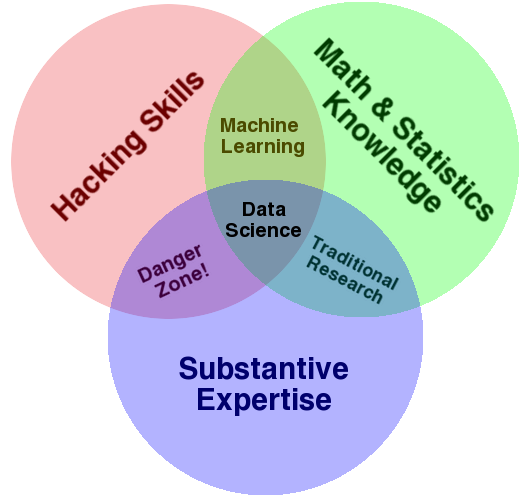
\includegraphics[width=7cm]{./pic/Data_Science_VD.png}
 \caption{\label{img:venn} Venn Diagram describing the different combination of skills used by a Data Scientist (by Drew Conway)}
\end{figure}

\begin{figure}[H]
 \centering
 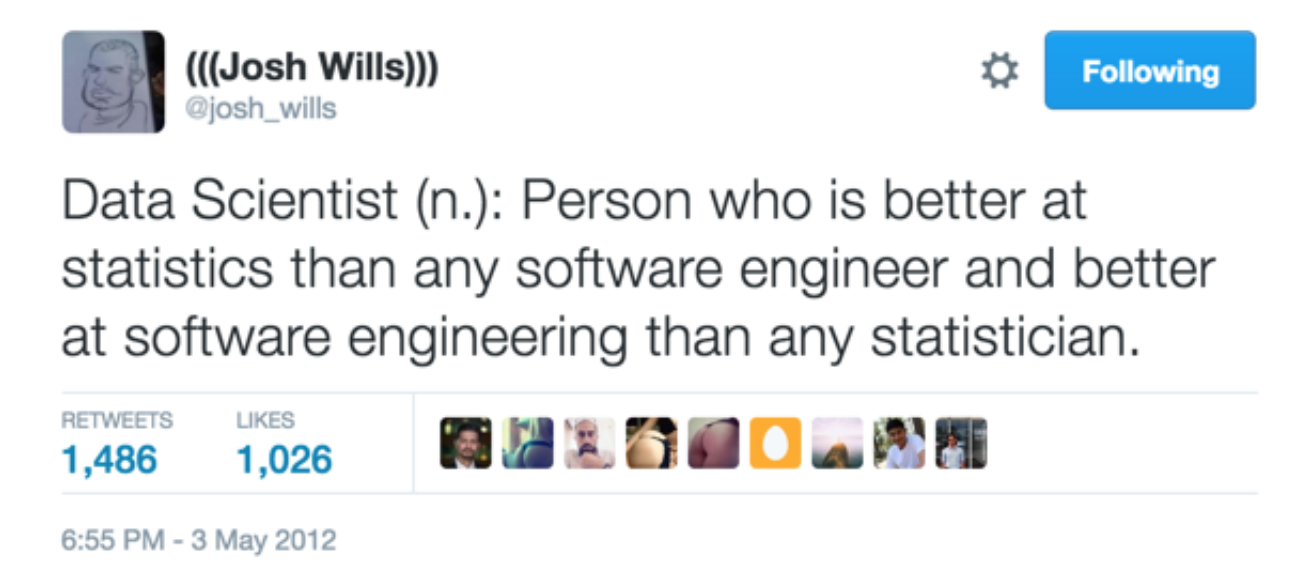
\includegraphics[width=10cm]{./pic/tweet_wills.png}
 \caption{\label{img:tweet_wills} A tweet from Josh Wills, Data Scientist at Slack.}
\end{figure}

{\bf A practical definition of Data Science} 

Data Science is about the whole processing pipeline to extract information out of data. As such, a Data Scientist {\bf understands and cares about the whole data pipeline}.

\begin{minipage}{0.5\textwidth}
\begin{figure}[H]
 \centering
 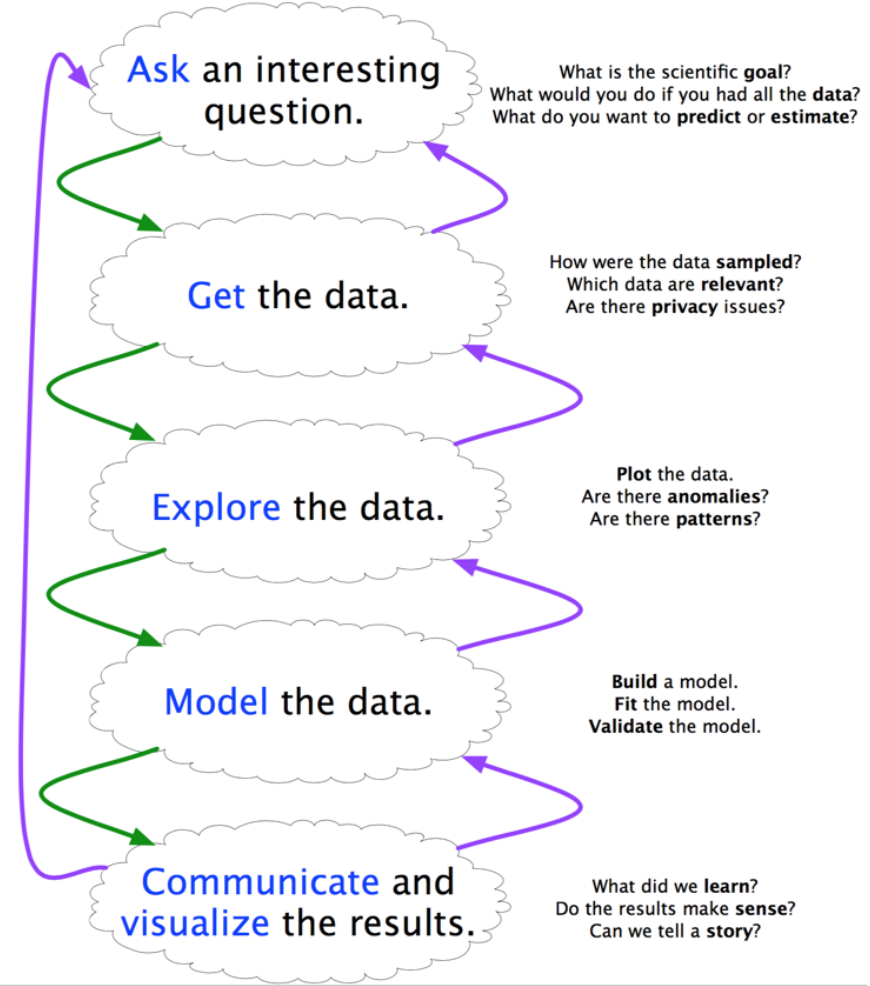
\includegraphics[width=8cm]{./pic/pipeline.png}
\end{figure}
\end{minipage} \hfill
\begin{minipage}{0.45\textwidth}
A {\bf data pipeline} consists of 3 steps:
\begin{enumerate}
 \item Preparing to run a model. \\
  {\it Gathering, cleaning, integrating, restructuring, transforming, loading, filtering, deleting, combining, merging, verifying, extracting, shaping}
 \item Running the model
 \item Communicating the results
\end{enumerate}
\vspace{0.5cm}
 A ``good'' Data Scientist will always go back and forth between the steps. The diagram on the left shows exactly what can happen. 
\end{minipage}
\\ \\
In this course, you will develop the following skills:
\begin{description}
 \item[data muning/scraping/sampling/cleaning] in order to get an informative, manageable data setlength
 \item[data storage and management] in order to be able to access data quickly and reliably during subsequent analysis
 \item[exploratory data analysis] to generate hypotheses and intuition about the data
 \item[prediction] based on statistical tools such as regression, classification, and clustering
 \item[communication of results] through visualization, stories and interpretable summaries
\end{description}


% ================ Definition ==============
% maybe to be moved at the end if it becomes a dictionnary
\section{Basic concepts}

A data science student is attended to understand the \textbf{Grammar of Data Science}. Having some backgrounds in SQL concepts is also a good thing because, as it is very common, people loves to make example with it. Here is a brief refresh of some definitions and concepts about data science.

\begin{itemize}
 \item {\bf Structured data} requires two key concepts:
 \begin{itemize}
  \item {\bf Data model} is a collection of concepts for describing data.
  \item {\bf Schema} is a description of a particular collection of data, using a given data model.
 \end{itemize}
 \item The {\bf Relational model} is on of the most common approach to manage data (SQL like) and can handle most of the data. A counter example is the facebook-like data which requires {\bf graph model}. This model is made of 2 parts:
 \begin{itemize}
  \item The {\bf Schema}. \\ For example, \verb+Students(sid: string, name:string, age:integer)+
  \item The {\bf Instance}, {\it i.e.} the data at a given time. \\
  Definitons:
  \begin{itemize}
   \item {\bf Cardinality} is the number of rows. (Number of items)
   \item {\bf Degree} or {\bf Arity} is the number of fields. (Number of attributes)
  \end{itemize}
 \end{itemize}
 \item Definitions of some ``Database'' terms:
 \begin{itemize}
  \item A {\bf JOIN} is a mean to combine tables based on shared attributes (most of the time some \textbf{IDs}). Despite its apparent simplicity beware of the many ways to compute a JOIN and check what is the default JOIN of a language before using it. The FIG \ref{join_SQL} summarises these possibilities.
  \item \textbf{Aggregation}, \textbf{reduction}, and {\bf groupby} are the action of reducing data with a common opperation (\textbf{sum}, \textbf{count}, \textbf{average}, ...) to summarise them. 
 \end{itemize}
 \item Definitions of some ``Pandas'' terms:
 \begin{itemize}
  \item {\bf Series} are a name, ordered dictionary
  \begin{itemize}
   \item keys are indexes
   \item built on \textbf{numpy.ndarray} (so values can be any Numpy data type)
  \end{itemize}  
  \item \textbf{DataFrame} is a table with named column
  \begin{itemize}
   \item the columns are series
   \item it is indeed a dictionary with (columnName $\rightarrow$ series)
  \end{itemize}  
 \end{itemize}
\end{itemize}

\begin{figure}%---------------FIG--------------
 \centering
 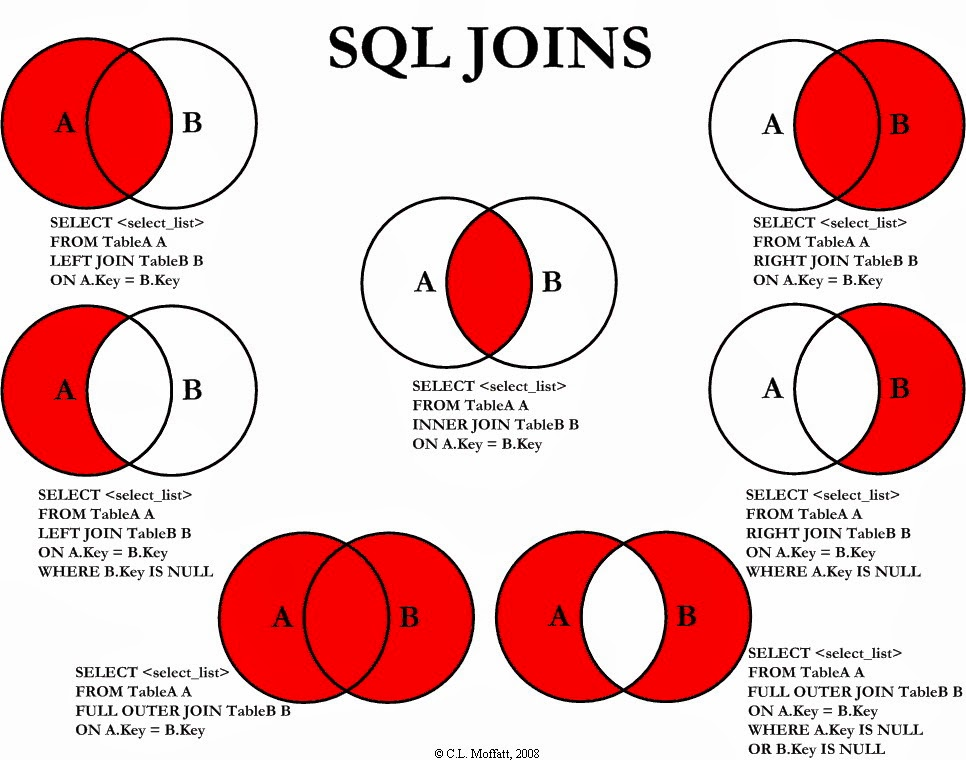
\includegraphics[width=12cm]{./pic/SQL_joins}
 \caption{\label{join_SQL} Different ways to join two tables and the related SQL command.}
\end{figure}


\subsection{Panda vs SQL}

Panda is built to allow easy and fast \textbf{data exploration} and not to be a database manager, as SQL is. Thus there are benefits and drawbacks of using it.


\begin{center} %---------------TAB--------------
\begin{tabular} {| l | l |}
\hline
\bf Pros & \bf Cons \\ \hline
Lightweight \& fast & Tables stored directly in memory \\
Great expressivness (combine SQL + Python) & No post-load indexing functionality\\
Easy plot for data visualization (eg Matplotlib) & No transactions, journalings\\ 
& Large, complex joins are slower \\ \hline
\end{tabular}
\end{center}

\subsection{OnLine Analytical Processing (OLAP cubes)}

OLAP tools enable users to analyze multidimensional data interactively from multiple perspectives. Conceptually, it is like an n-dimensional spreadsheet (a cube) on which we can apply various opperations to take decisions.

OLAP cubes are an other way to see data table and are contructed based on them, as shows FIG \ref{OLAP_cubes}.

\begin{figure}[H]%---------------FIG--------------
 \centering
 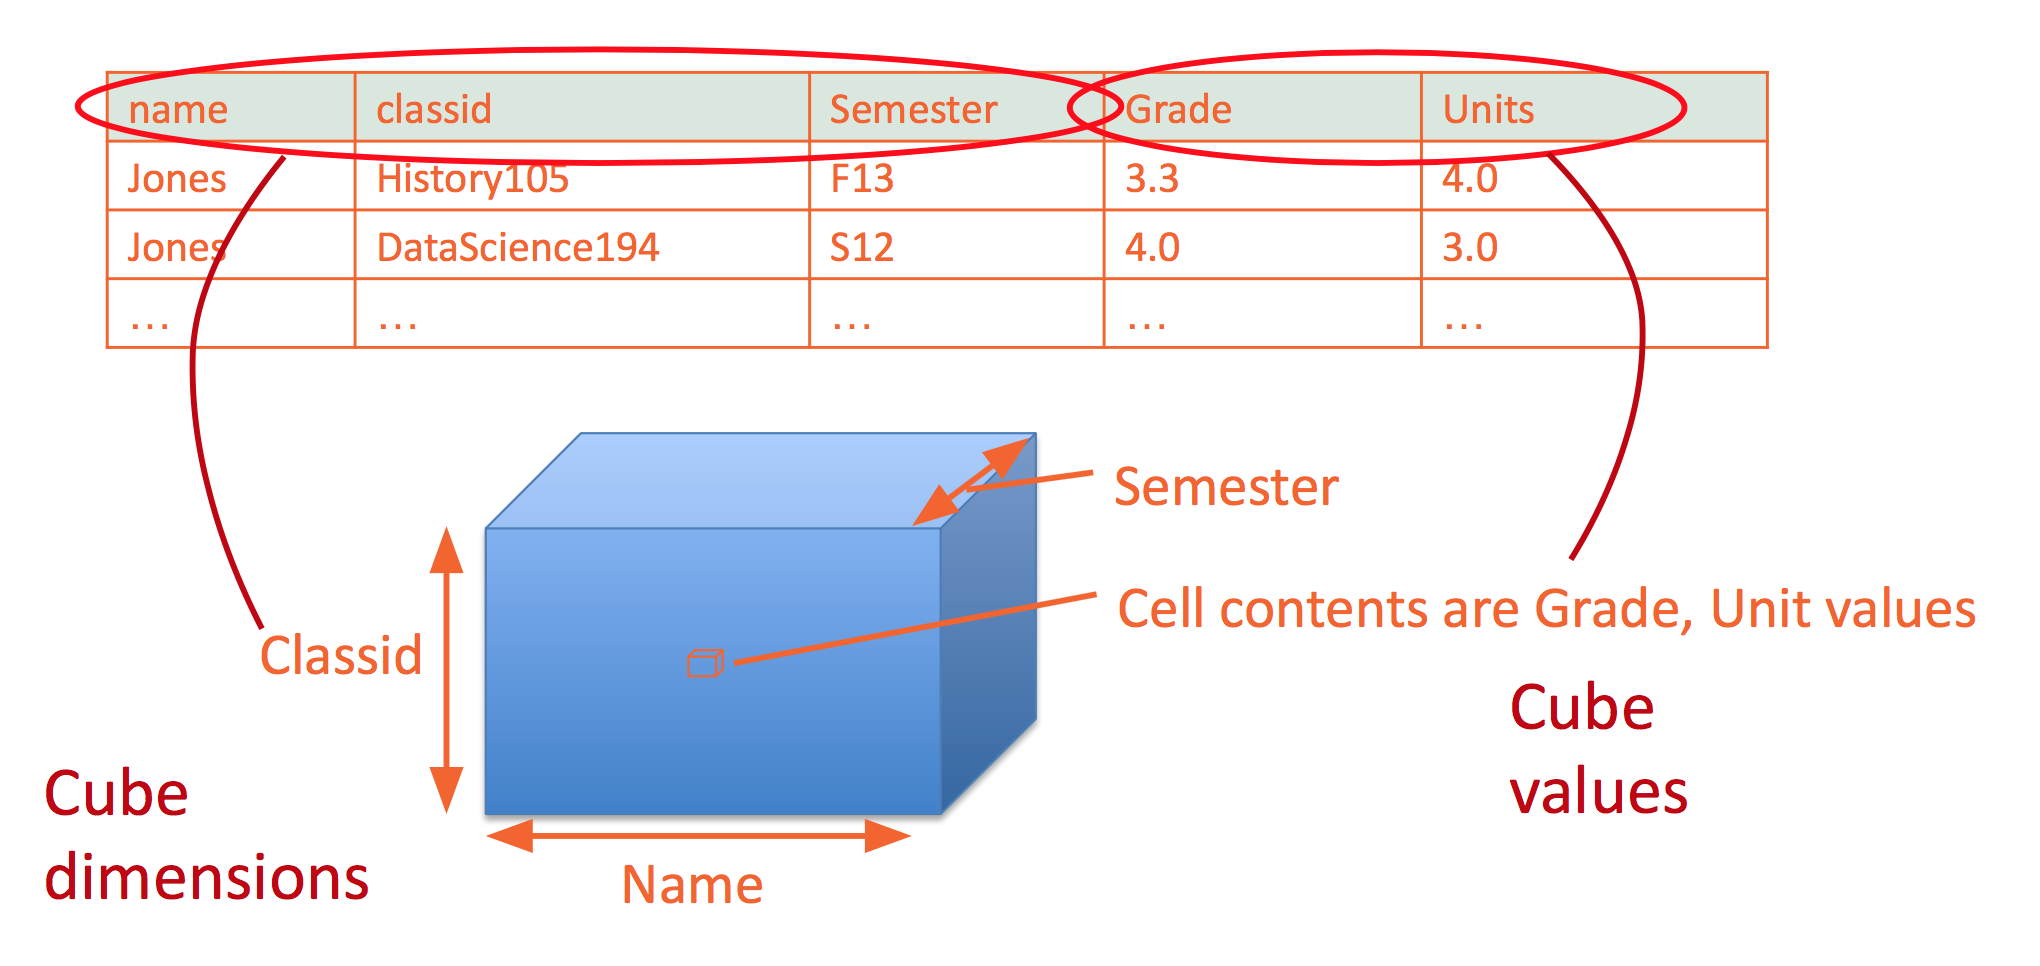
\includegraphics[width=12cm]{./pic/OLAP_cube}
 \caption{\label{OLAP_cubes} Construction of an OLAP cube from a table.}
\end{figure}

Operations on OLAP cubes are the following and are illustrated on FIG \ref{OLAP_operations}
\begin{itemize}
	\item \textbf{Slicing} fixes one or more variable
	\item \textbf{Dicing} selects a range of one or more variable
	\item \textbf{Driling up/down} changes levels of a hierarchically-indexed variable, ie "zoom" on a variable and see the sub-categories it contains.
	\item \textbf{Pivoting} change the point of view of the cube. Swap an aggregated variable an a detailed one.
\end{itemize}

\begin{figure} [h] %----------- SubGraph ---------------------
\centerline{
\subfigure[Slincing\label{olap_slicing}] {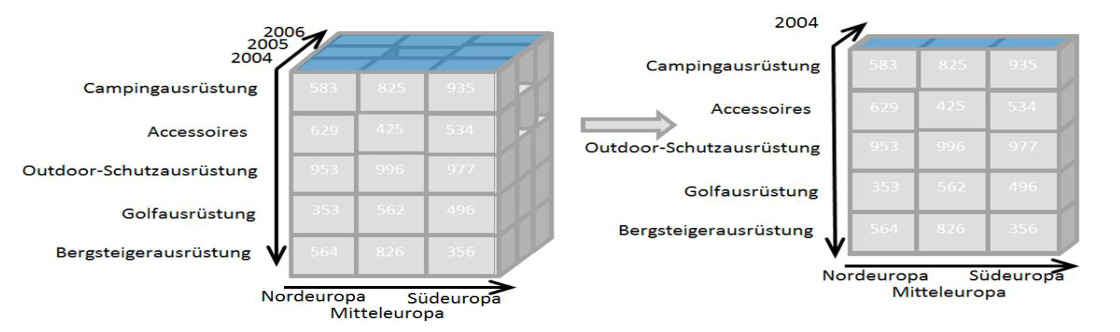
\includegraphics[width=7cm]{pic/Slicing} }
\subfigure[Dicing\label{olap_dicing}] {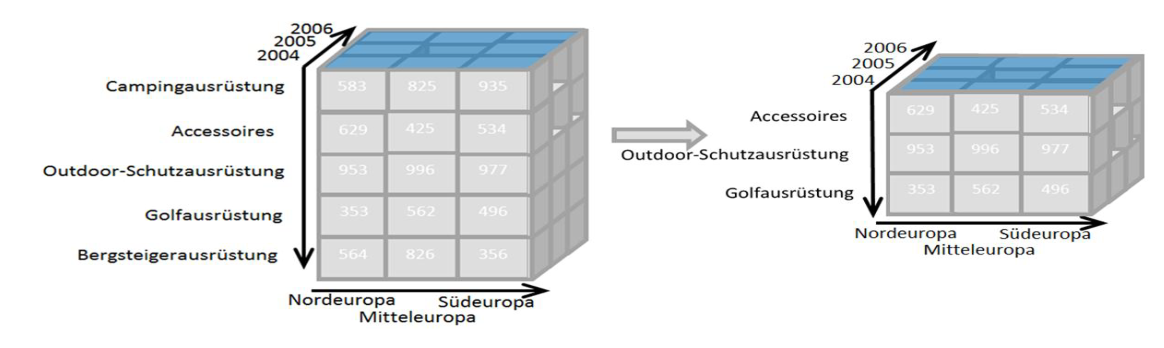
\includegraphics[width=7cm]{pic/Dicing} } 
}
\centerline{
\subfigure[Driling up/down\label{olap_driling}] {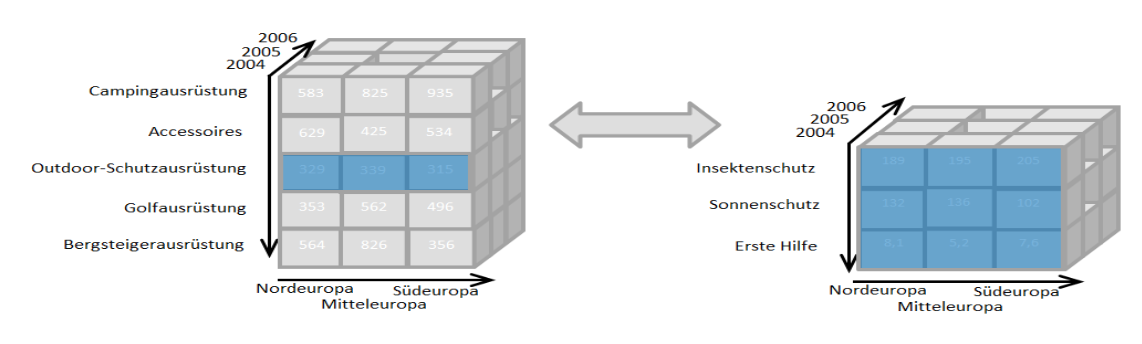
\includegraphics[width=7cm]{pic/Drilling_up_down} }
\subfigure[Pivoting\label{olap_pivoting}] {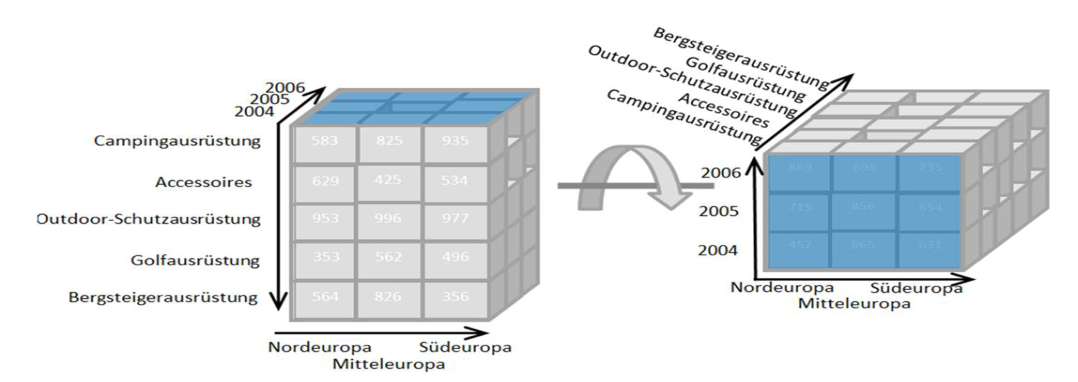
\includegraphics[width=7cm]{pic/Pivoting} } 
}
\caption{\label{OLAP_operations} Operations on OLAP cubes} 
\end{figure}

\begin{center} %---------------TAB--------------
\begin{tabular} {| l | l |}
\hline
\bf Pros & \bf Cons \\ \hline
& \\
\parbox[t][][t]{7cm}{The main adventage of OLAP cubes is that their are \textbf{conceptualy simpler} to understand by a non-scientist person, eg a business man who have to take day-to-day decisions based on company's data. Aggregations are limited but cover the main common cases that we can encounter.
}&
\parbox[t][][t]{7cm}{Because of the "on-line" behaviour of this approach, all type of aggregation must be pre-calculated amoung all combination of axis which is very \textbf{expensive in memory and in time} (when updating the data)}\\
& \\
\hline
\end{tabular}
\end{center}

% ================ Data Wrangling ==============
\section{Data Wrangling}

\begin{figure}[H]%---------------FIG--------------
 \centering
 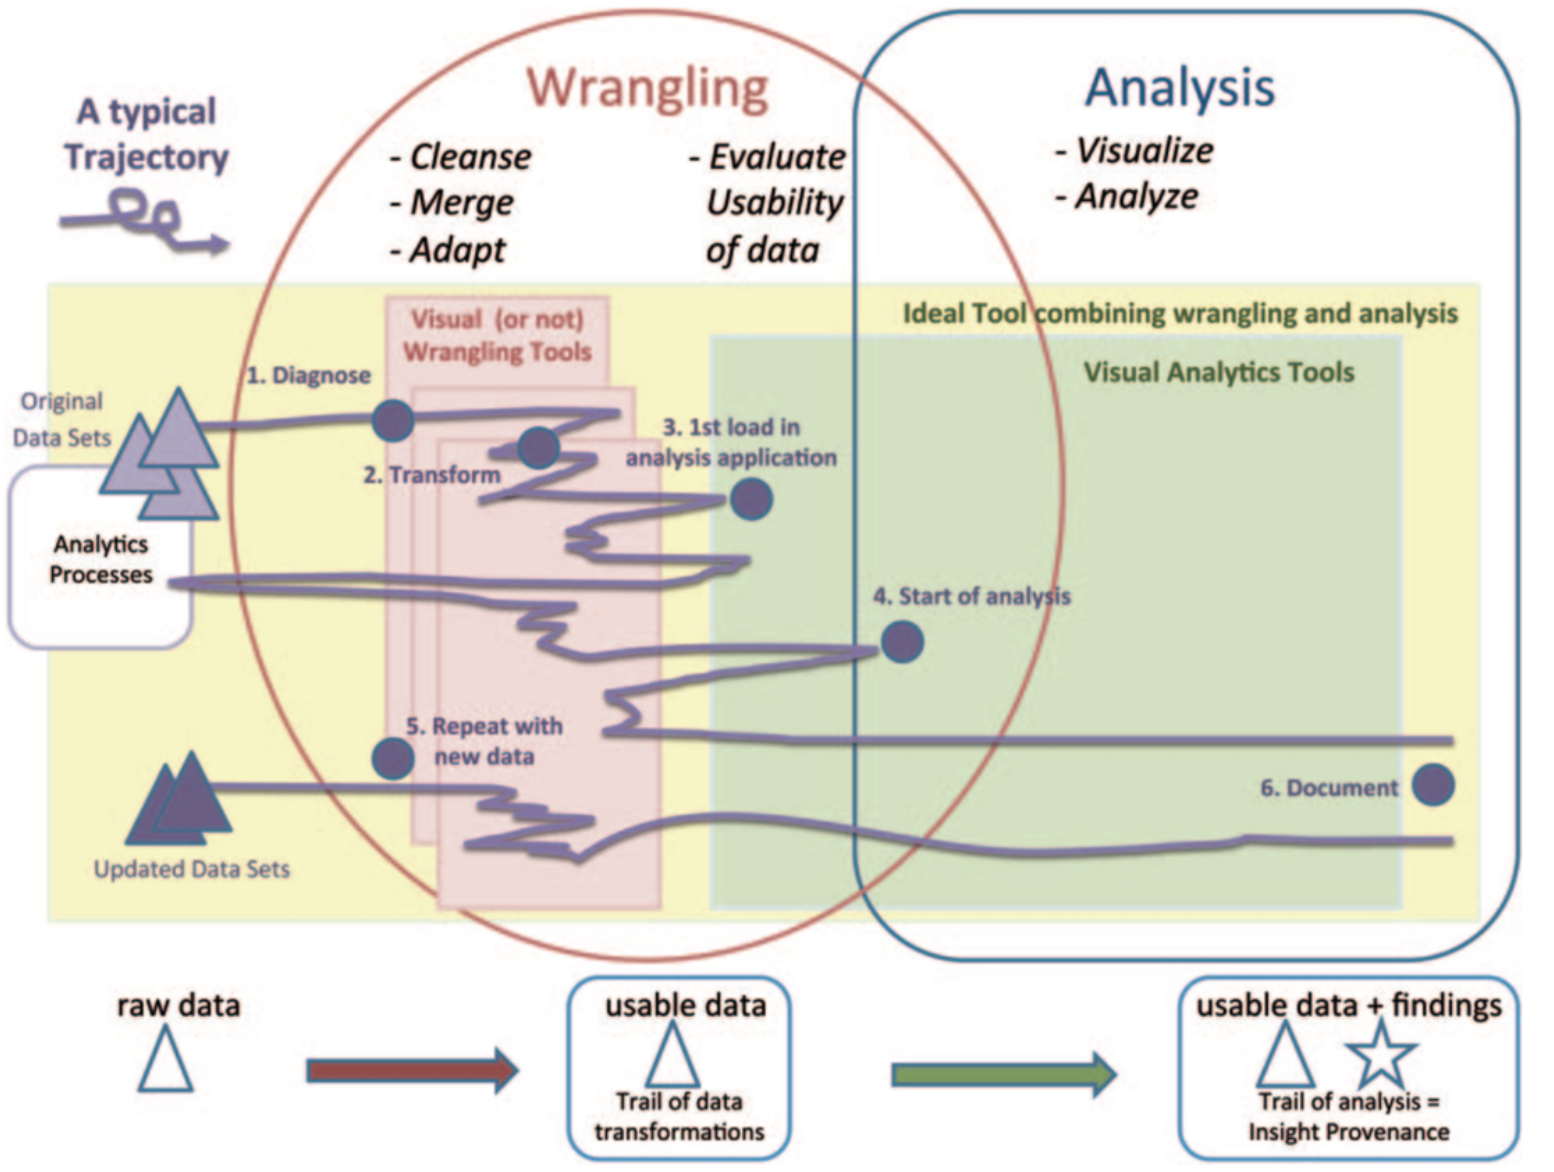
\includegraphics[width=12cm]{./pic/path_data_wrangling}
 \caption{\label{path_data_wrangling}Things do not always happen as expected...}
\end{figure}

Before any analysis, data need to be transformed from "dirty" to clean and processable data. 

Data comes from different sources (excel or SQL?), sometime collected through different methods over time, with different conventions (space or NaN?), etc ... Data wrangling's goal is to \textbf{extract and standardize these raw data}. The best way to do it is to \textbf{combine automation with visualizations} in order to find outliers. 

Data's problem can come from (non-exhaustive): 
\begin{itemize}
  \item Missing data
  \item Incorrect data
  \item Inconsistent representations of the same data
  \item Non-standardized data (centimeter or inches? farenheit or celsuis ?)
  \item Duplicated data
\end{itemize}

About 75\% of theses problem will need \textbf{human intervention} to be corrected (by the data-scientist or by crowdsourcing).

Even if it seems really dirty, \textbf{beware not to over-sanitize the data!}. Applying what we can call "defensive programming" is not a good idea because we risk to lose any interesting data, keeping only the ones that fit perfectly in our model.

\subsection{Diagnosis of the data}

One of the most important aspect of Data Wrangling is to {\bf understand} the data and to {\bf find possible problems}. In order to ``diagnose'' the data, two tools can be used:
\begin{itemize}
 \item {\bf Visualization} (A {\it toughtful} visualization will always help)
 \item {\bf Basic Statistics} 
\end{itemize}

Matrix visualizations of the facebook graph is shown in Figure \ref{pic:fb}. The Relational visualization, Figure \ref{pic:fb1}, does not show any particular problem in the data. But the Time dependant visualization, Figure \ref{pic:fb2}, shows that the Facebook API reached its limit while collecting data.

\begin{figure} [h] %----------- SubGraph ---------------------
\centerline{
\subfigure[Relational visualization \label{pic:fb1}] {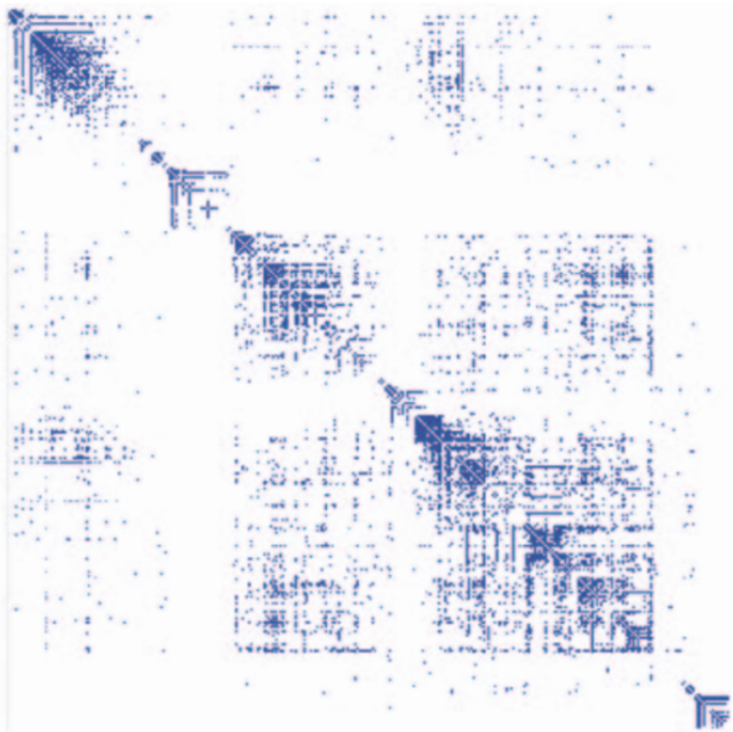
\includegraphics[width=7cm]{pic/fb1} }
\subfigure[Time dependant visualization\label{pic:fb2}] {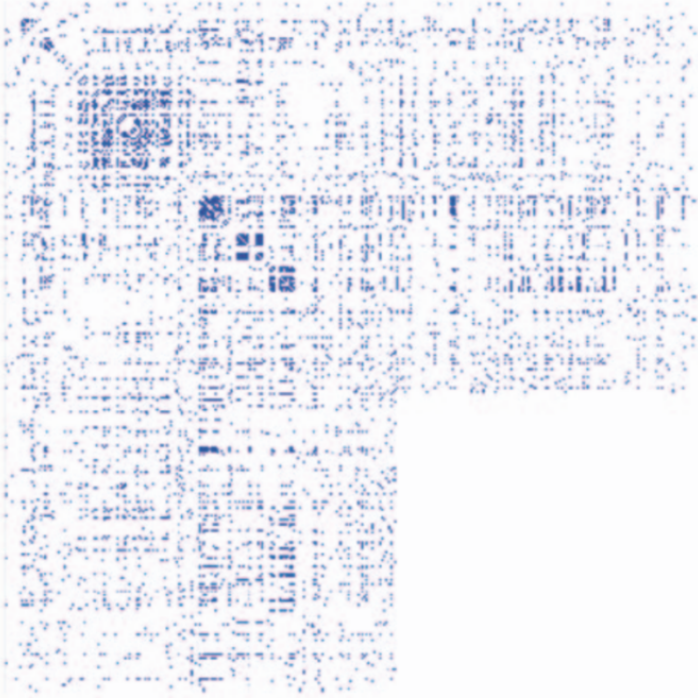
\includegraphics[width=7cm]{pic/fb2} } 
}
\caption{\label{pic:fb} Matrix visualization of the facebook graph.} 
\end{figure}


\subsection{Dealing with missing values}

Values can often miss from the data we have, because of various events (war, fire, ...). We must detect and correct these values with different method according with the domain we are working in.

Whatever the method used, it's good to keep track of these changes to know which are original data and which are modified ones.

\begin{itemize}
  \item Set values to zero FIG \ref{miss_val}(a)
  \item Interpolate based on existing data FIG \ref{miss_val}(b)
  \item Omit missing data FIG \ref{miss_val}(c)
  \item Interpolation with track kept \ref{miss_val}(d)
\end{itemize}

\begin{figure}[H]%---------------FIG--------------
 \centering
 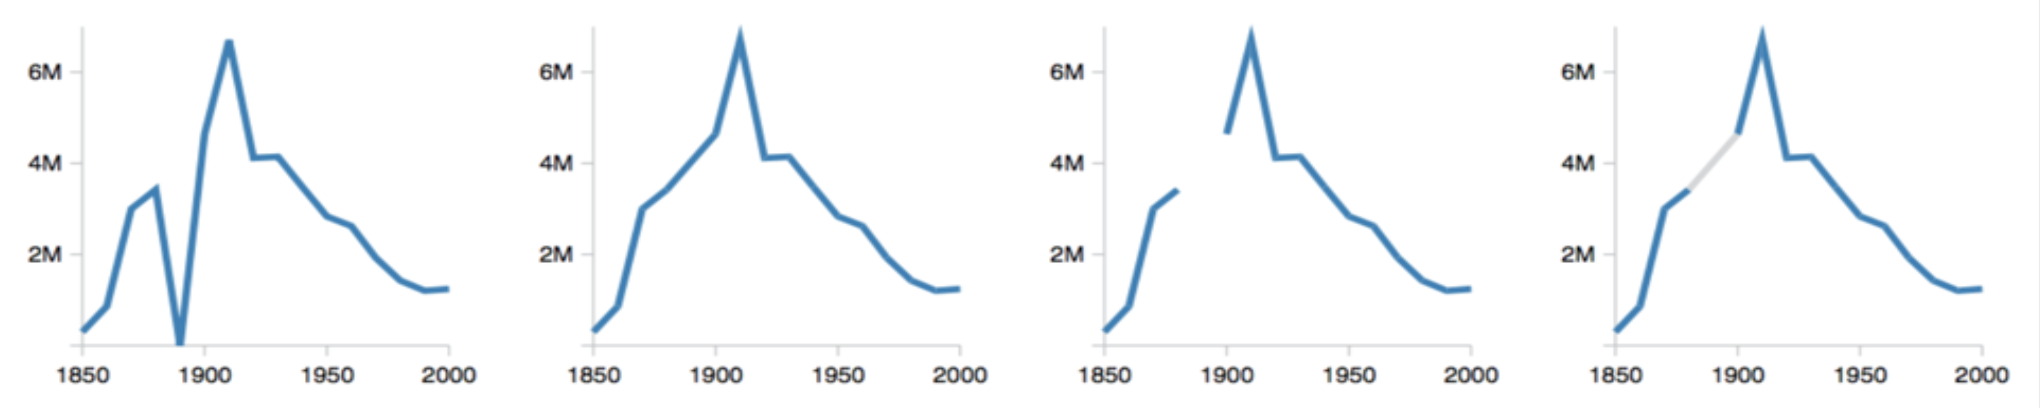
\includegraphics[width=15cm]{./pic/missing_values}
 \caption{\label{miss_val}To deal with missing values.}
\end{figure}

\subsection{General procedure}

Once the data are well wrangled and before trying to analyse them we must take care of two more steps:

\begin{enumerate}
  \item \textbf{Deal with uncertain data} (can arise from measurement errors, wrong sampling strategies, etc.)
  \item \textbf{Parse/trasform data} (with aggregation and reduction techniques) to obtain meaningful records
\end{enumerate}
 
It's always ideal to have the code and/or the documentation about the dataset you are analyzing (provenance).
 
% ================ Data Variety ==============
\section{Data Variety}

The ``3 Vs'' of Big Data: {\it Volume}, {\it Velocity} and {\bf Variety}. A course on Database will cover the {\it Volume} and {\it Velocity} parts. In this course, we try to figure out how to address the {\bf Variety} part.
\\\\
{\bf ETL}:
\begin{itemize}
 \item {\bf Extract} from the {\it source(s)}.
 \item {\bf Load} data into the {\it sink}. 
 \item {\bf Transform} data at the source, sink, or in a {\it staging area}.
\end{itemize}
Semi-structured data: no strict structure, but some info are given. => Data range comes from very structured data in DB to totally unstructered data such as web pages.
\\\\
Traditional DB are {\bf schema-on-write}. (You can't load data into a table without a schema!) But NoSQL (Next generation) DB are {\bf schema-on-read} or {\bf schemaless}. You can either avoid having a schema or have a schema only when you read data. Examples of schemaless: Youtube, Google Cache.
\\\\
Schema-on-write data type: SQL
Schema-rn-read data type: XML (when stored without a schema, the numerical data is stored as {\bf strings}) Using a parser, we can return a typed data. (Faster because number not string + can make checks. => Type is good)
\\\\
XML and {\bf DOM} (Document-Object Models). Every webpage on internet becomes a DOM. Tree-structured. 
XML QUeries: allows a DB to interpret data when running queries, {\it i.e.} to do {\bf arithmetic} or {\bf range queries} on the numerical values. (With or without a schema)
\\\\
{\bf JSON} (Javascript Object Notation) Totally schemaless. But we can also use with schema. It's used to represent {\bf hierachical data structures} directly in the languages. (Lot of libraries to do that). Transformation on the data are {\bf \color{red} procedural} in the target language. Easier for some tasks, but painful for e.g. schema changes.
\\\\
Data Tools:
\begin{itemize}
 \item {\bf XML}
 \begin{itemize}
  \item Separation between schema and data.
  \item Data can be represented and stored without schema (as strings).
  \item More verbose (but not true after compression or in DB).
  \item Standard Query/Transformation languages XSLT and Xquery.
 \end{itemize}
 \item {\bf JSON}
 \begin{itemize}
  \item Types inferred inline. Schema rarely used but can be.
  \item Data without schema uses type inference (string, int, float, ...).
  \item More succinct in ASCII form.
  \item Transformation/ingestion rely on code (Java or Javascript).
 \end{itemize}
\end{itemize}

{\bf Tabular Data} -> CSV or TSV
Description of a table: 
- A {\bf table} is a collection of {\bf rows} and {\bf columns}
- Each row has an {\bf index}
- Each column has a {\bf name}
- A {\bf cell} is specified by (index, name) pair
- A cell may or may not have a {\bf value}
Schema = (minimal) column types) 
\\\\
Sensors output data in the form of time series -> tabular data. Systems dealing with sensor data should
\begin{itemize}
 \item support both long-term ({\bf trend}) and short-term ({\bf real-time}) queries
 \item have {\bf low latency} but also efficient, real-time indexing for longer-term queries
 \item support triggers (alerts) for a variety of conditions
\end{itemize}
{\bf \color{red} Complexity of data format does not determine complexity of the system required to handle it. -> Stock market}
\\\\
{\bf Log Files}
Processes, usually daemons, create logs. (https, mysqld, syslogd, ...)
Syslog - Standard for System messages. Enables rich analysis. ``Spelunking'' for bugs -> Splunk: Monitor ressources many machines. 
\\\\
{\bf Processing XML and JSON}
DOM is an easy object to work with: all the data is accessible by links once it's in the memory. The problem is that I might not care about most of the data => we might {\bf not be able to fit the DOM for a large object in RAM}.
\\\\
{\bf SAX}: Event-Driven Parsing. Helps to deal with Big Data. Exists with pretty much any format that exists. It finds all the {\bf open-close-tag events} in an XML documents, and {\bf does callbacks to user code}.

Pros:
+ User code can respond to only a subset of events corresponding to the tags.
+ User code cna correctly computer aggregates from the data rathen than create a record for each tag.
+ User code can implement felxible error recovery strategies for ill-formed XML
- User code must implement a state machine to keep track of ``where it is'' in the DOM tree.
\\\\
Most JSON parsers construct the ``DOM'' directly. Sometimes SAY-style is the only way to handle ill-formed dataset (endless array of objects)
\\\\
{\bf Binary formats}
Often the key to performance, {\bf avoiding expensive parsing}! Modern formats support nested structures, various levels of schema enforcement, {\bf compression}, etc. {\bf \color{red} Consider converting to one of those formats at the beginning of your processing pipeline (especially on a project with Big Data!)}
\begin{itemize}
 \item Protocol Buffers (Goggle)
 \item Avro (supports schema evolution)
 \item Parquet (column oriented, first-class citizen in Spark)
 \item etc.
\end{itemize}
{\bf HTML}
Common Crawl has 0.1\% of Google's web crawl. Because Google can scrape data which are behind the form (hidden link, authentication, forms, etc.) using their technology. Common Crawl just uses a simple ``algorithm'' to extract links.
\\
List and describe in one line the different HTML stuff. WikiData, schema.org, etc. 
\\\\
{\bf Web Services}
Large web sites discourage to do screen-scraping. User Web Service APIs. This is the {\bf right} was to get data from online sources.
\\
{\bf W3C}: A ``Web service'' is ``a software system designed to support interoperable machine-to-machine interaction over a network''. Two kinds:
- XML-base RPC-style messages: SOAP
- REST-stly stateless interactions, URLs encode state.
\\\\
{\bf REST}: REpresentation State Transfer
DEFINITION HERE! slide 47-48
\\\\
{\bf REST vs RPC}



%======= TABLEAU ===========
%\begin{center} %---------------Tab--------------
%\begin{tabular} {| c | c | c | c | c | c |}
%\hline
 %& & & & & $\\ \hline
%\end{tabular}
%\end{center}


%===========GRAPH================
%\begin{figure} %---------------------Graph---------------------------
%\begin{center}
%\includegraphics[width=12cm]{graph/ampli2} 
%\end{center}
%\caption{\em  \label{label}
%L�gende
%}
%\end{figure}


%========SUBGRAPH=======
%\begin{figure} [h] %----------- SubGraph ---------------------
%\centerline{
%\subfigure[ sublegend ] {\label{sfig:thetat} \includegraphics[width=7cm]{ graph/graph_convdt3 } }
%\subfigure[ sublegend ] {\label{sfig:thetafin} \includegraphics[width=7cm]{ graph/graph_convtfin } } 
%}
%\caption{\label{ label } 
%L�gende
%} 
%\end{figure}








\end{document} %%%% THE END %%%%
